\subsection{Виджет выбора даты и времени}
\label{widget:date_time_picker}
Вызов данного виджета производится путём нажатия на кнопку \vcenteredinclude[height=25px]{images/widgets/date_time_picker_call_btn}, после чего на экране появится календарь, в котором пользователь может задать дату.
Для переключения на виджет задания времени, пользователю необходимо нажать на кнопку \vcenteredinclude[height=25px]{images/widgets/date_time_picker_time_btn}, после чего отобразится виджет выбора времени.

\subsection{Виджет загрузки файлов}
\label{widget:file_upload}
Для асинхронной загрузки файлов на сервер используется виджет загрузки файлов. Слева под меткой поля показано текущее загруженное изображение, если оно есть (см рис.~\ref{img:widgets:file_upload_ok}) или изображение по умолчанию, если ничего не загружено (см рис.~\ref{img:widget:file_upload_default_logo}). 

\begin{figure}[H]
	\center{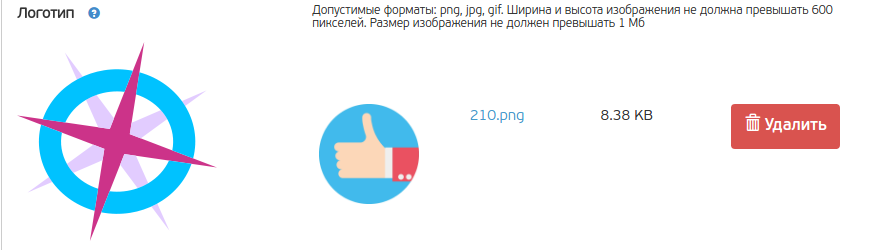
\includegraphics[width=1\linewidth]{images/widgets/file_upload_ok}}
	\caption{Успешная загрузка файла}
	\label{img:widgets:file_upload_ok}
\end{figure}

\begin{figure}[H]
	\center{
\includegraphics[width=1\linewidth]{images/widgets/file_upload_default_logo}}
	\caption{Файловое поле с изображением по умолчанию}
	\label{img:widget:file_upload_default_logo}
\end{figure}

Для того чтобы начать загрузку файла, необходимо нажать на кнопку \vcenteredinclude[height=25px]{images/widgets/file_uploat_select_file} и в окне проводника выбрать желаемый файл. Загружаемый файл должен соответствовать ограничениям на формат и размерам указанным справа от метки поля, в противном случае появится сообщение об ошибке.

\subsection{Виджет определения порядка следования записи}
\label{widget:ordering}
Виджет определения порядка следования записи представляет из себя список, элементы которого можно менять местами. Изменить порядок можно, перетащив выбранную строку на новую позицию при помощи мыши (см. рис.~\ref{img:widgect:ordered_list}).

\begin{figure}[H]
	\center{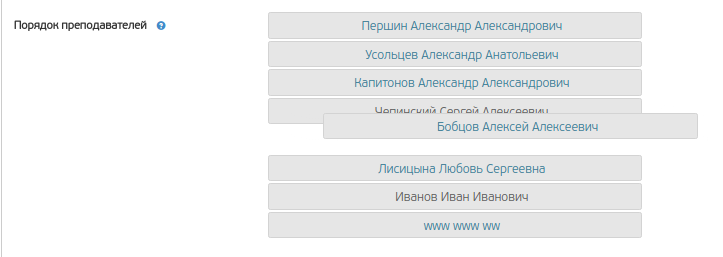
\includegraphics[width=1\linewidth]{images/widgets/ordered_list}}
	\caption{Виджет определения порядка следования записи}
	\label{img:widgect:ordered_list}
\end{figure}

В ряде случаев элементы списка можно удалять, нажав на кнопку \vcenteredinclude[height=25px]{images/widgets/delete_btn}.

\subsection{Виджет выпадающего списка с автодополнением}
\label{widget:autocomplete}
Виджет выпадающего списка предназначен для упрощения поиска. Внешний вид виджета представлен на рисунке~\ref{img:widgect:autocomplete_view} (в ряде случаев на виджете может присутствовать подсказка). При нажатии на виджет появится список значений, которые могут быть заданы в этом поле (рис.~\ref{img:widgect:autocomplete_open_view}).
\begin{figure}[H]
	\center{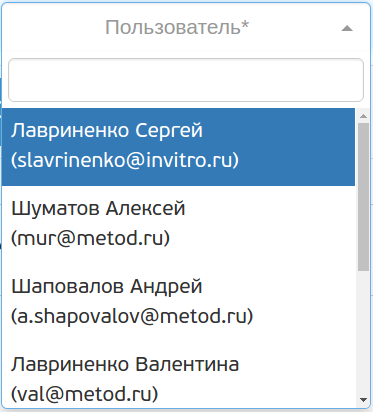
\includegraphics[width=0.5\linewidth]{images/widgets/autocomplete_open_view}}
	\caption{Внешний вид виджета при нажатии на него}
	\label{img:widgect:autocomplete_open_view}
\end{figure}

Имеется возможность фильтрации результатов путем ввода с клавиатуры части названия. Выбор необходимого результата осуществляется щелчком указателя мыши по нужному элементу в списке или по нажатию клавиши \keys{\enter} (в последнем случае будет выбран выделенный элемент списка). Для того что бы отменить выбор, необходимо нажать клавишу \keys{\esc} или кликнуть курсором мыши вне виджета. Очистка поля производится нажатием на \quotes{X}.
